\documentclass{article}

\usepackage[latin1]{inputenc}
\usepackage{tikz}
\usepackage{pgfplots}
\usetikzlibrary{backgrounds}

% GNUPLOT required
\begin{document}
\pagestyle{empty}

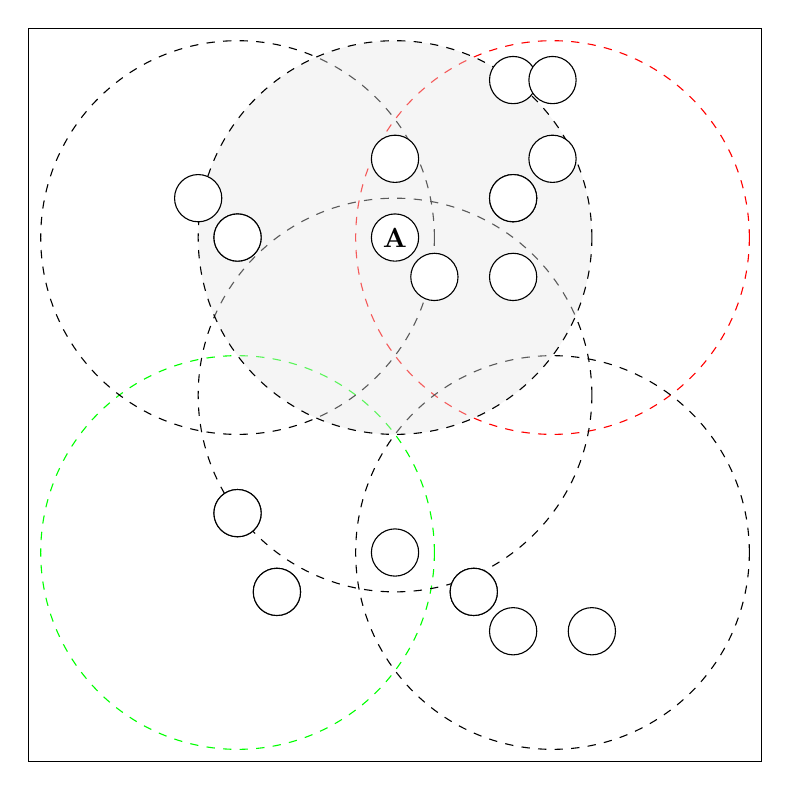
\begin{tikzpicture}[framed]
\draw[dashed, red] (2, 2) circle [radius=2.5];
\draw[dashed, green] (-2, -2) circle [radius=2.5];
\draw[dashed, black] (2, -2) circle [radius=2.5];
\draw[dashed, black] (-2, 2) circle [radius=2.5];
\draw[dashed, black] (0, 0) circle [radius=2.5];
\draw[dashed, black, fill opacity=.4, fill=gray!20] (0, 2) circle [radius=2.5];
\draw[black, fill=white] (0, 2)  circle [radius=0.30] node {$\bf{A}$}; 
\draw[black, fill=white] (-2, 2)  circle [radius=0.30] ; 
\draw[black, fill=white] (-2.5, 2.5)  circle [radius=0.30] ; 
\draw[black, fill=white] (1.5, 4)  circle [radius=0.30] ; 
\draw[black, fill=white] (2, 3)  circle [radius=0.30] ; 
\draw[black, fill=white] (1.5, 2.5)  circle [radius=0.30] ; 
\draw[black, fill=white] (-2, -1.5)  circle [radius=0.30] ; 
\draw[black, fill=white] (1, -2.5)  circle [radius=0.30] ; 
\draw[black, fill=white] (0.5, 1.5)  circle [radius=0.30] ; 
\draw[black, fill=white] (-1.5, -2.5)  circle [radius=0.30] ; 
\draw[black, fill=white] (1.5, -3)  circle [radius=0.30] ; 
\draw[black, fill=white] (-2, 2)  circle [radius=0.30] ; 
\draw[black, fill=white] (0, 3)  circle [radius=0.30] ; 
\draw[black, fill=white] (0, -2)  circle [radius=0.30] ; 
\draw[black, fill=white] (2, 4)  circle [radius=0.30] ; 
\draw[black, fill=white] (1.5, 2.5)  circle [radius=0.30] ; 
\draw[black, fill=white] (-2, -1.5)  circle [radius=0.30] ; 
\draw[black, fill=white] (1, -2.5)  circle [radius=0.30] ; 
\draw[black, fill=white] (1.5, 1.5)  circle [radius=0.30] ; 
\draw[black, fill=white] (-1.5, -2.5)  circle [radius=0.30] ; 
\draw[black, fill=white] (2.5, -3)  circle [radius=0.30] ; 



\end{tikzpicture}


\end{document}